\section{Auswertung}\label{sec:auswertung}
Im folgenden Kapitel werden die aufgenommenen Messwerte ausgewertet.
\subsection{Überprüfen der Stabilitätsbedingung}
Wie in \autoref{subsubsec:stabilitaet} erläutert, ist Stabilität nur unter der Bedingung $g_1\cdot g_2\in[0,1)$ erfüllt. Für die verwendeten Spiegelkonfigurationen ist dies grafisch in \autoref{fig:stabil} dargestellt.
\begin{figure}[H]
    \centering
    \begin{subfigure}[b]{0.48\textwidth}
        \centering
        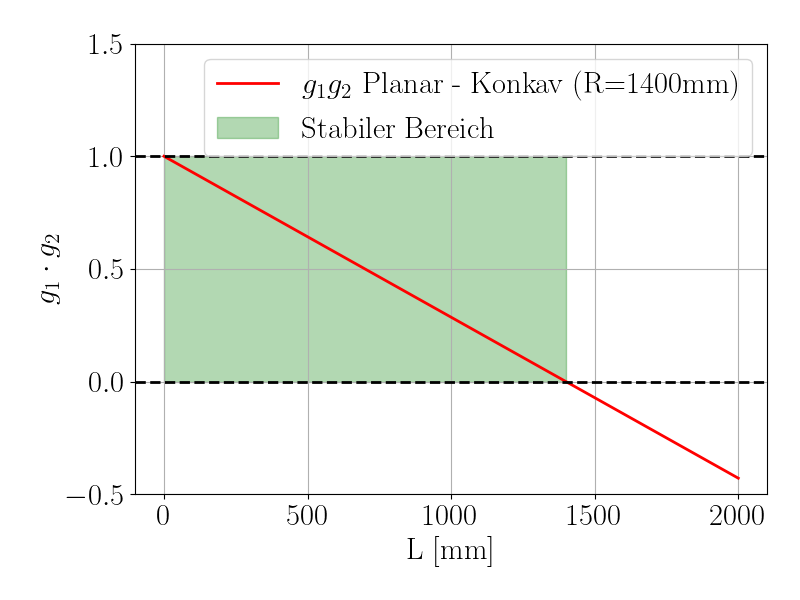
\includegraphics[scale=0.4]{Skripte/2000.png}
        \caption{Konkav-planare Konfiguration}
        \label{fig:kette_a}
    \end{subfigure}
    \hfill
    \begin{subfigure}[b]{0.48\textwidth}
        \centering
        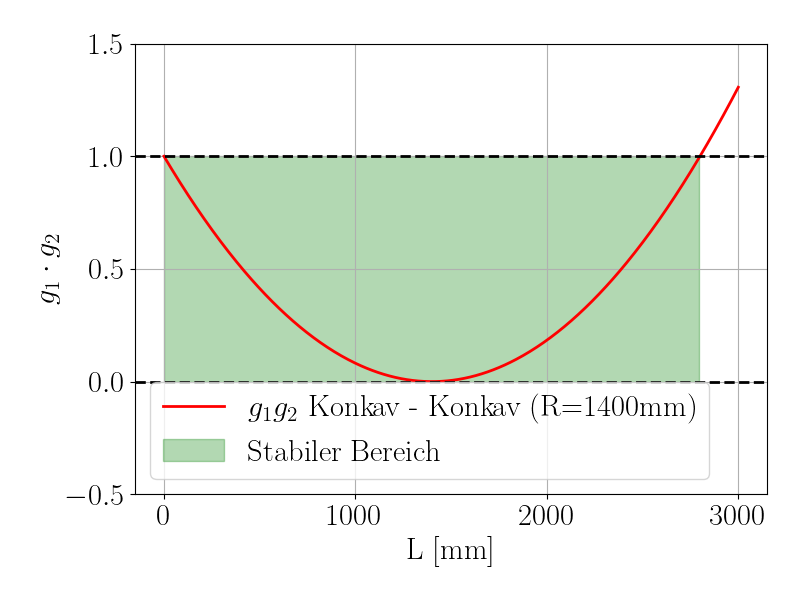
\includegraphics[scale=0.4]{Skripte/3000.png}
        \caption{Konkav-konkave Konfiguration}
        \label{fig:kette_b}
    \end{subfigure}
    \caption{Plot der Stabilitätsparameter für verschiedene Resonatorkonfigurationenmit grün hervorgehobenen stabilen Bereich}
    \label{fig:kette}
\end{figure}
Es ergeben sich die theoretischen Grenzwerte der Resonatorlänge von 
\begin{align}
    L_\text{max k-p}=R=1400
\end{align}
beziehungsweise 
\begin{align}
    L_\text{max k-k}=2\cdot R=2800\text{.}
\end{align}
Im Versuch konnte für den planar-konkaven Resonator eine maximale Länge von \SI{121}{\centi\meter} stabilisiert werden, für die konkav-konkave Kombination wurde die gesamte zur Verfügung stehende Schiene verwendet um eine Resonatorlänge von \SI{218}{\centi\meter} zu erreichen.
